% Options for packages loaded elsewhere
\PassOptionsToPackage{unicode}{hyperref}
\PassOptionsToPackage{hyphens}{url}
%
\documentclass[
]{article}
\usepackage{amsmath,amssymb}
\usepackage{lmodern}
\usepackage{iftex}
\ifPDFTeX
  \usepackage[T1]{fontenc}
  \usepackage[utf8]{inputenc}
  \usepackage{textcomp} % provide euro and other symbols
\else % if luatex or xetex
  \usepackage{unicode-math}
  \defaultfontfeatures{Scale=MatchLowercase}
  \defaultfontfeatures[\rmfamily]{Ligatures=TeX,Scale=1}
\fi
% Use upquote if available, for straight quotes in verbatim environments
\IfFileExists{upquote.sty}{\usepackage{upquote}}{}
\IfFileExists{microtype.sty}{% use microtype if available
  \usepackage[]{microtype}
  \UseMicrotypeSet[protrusion]{basicmath} % disable protrusion for tt fonts
}{}
\makeatletter
\@ifundefined{KOMAClassName}{% if non-KOMA class
  \IfFileExists{parskip.sty}{%
    \usepackage{parskip}
  }{% else
    \setlength{\parindent}{0pt}
    \setlength{\parskip}{6pt plus 2pt minus 1pt}}
}{% if KOMA class
  \KOMAoptions{parskip=half}}
\makeatother
\usepackage{xcolor}
\usepackage[margin=1in]{geometry}
\usepackage{color}
\usepackage{fancyvrb}
\newcommand{\VerbBar}{|}
\newcommand{\VERB}{\Verb[commandchars=\\\{\}]}
\DefineVerbatimEnvironment{Highlighting}{Verbatim}{commandchars=\\\{\}}
% Add ',fontsize=\small' for more characters per line
\usepackage{framed}
\definecolor{shadecolor}{RGB}{248,248,248}
\newenvironment{Shaded}{\begin{snugshade}}{\end{snugshade}}
\newcommand{\AlertTok}[1]{\textcolor[rgb]{0.94,0.16,0.16}{#1}}
\newcommand{\AnnotationTok}[1]{\textcolor[rgb]{0.56,0.35,0.01}{\textbf{\textit{#1}}}}
\newcommand{\AttributeTok}[1]{\textcolor[rgb]{0.77,0.63,0.00}{#1}}
\newcommand{\BaseNTok}[1]{\textcolor[rgb]{0.00,0.00,0.81}{#1}}
\newcommand{\BuiltInTok}[1]{#1}
\newcommand{\CharTok}[1]{\textcolor[rgb]{0.31,0.60,0.02}{#1}}
\newcommand{\CommentTok}[1]{\textcolor[rgb]{0.56,0.35,0.01}{\textit{#1}}}
\newcommand{\CommentVarTok}[1]{\textcolor[rgb]{0.56,0.35,0.01}{\textbf{\textit{#1}}}}
\newcommand{\ConstantTok}[1]{\textcolor[rgb]{0.00,0.00,0.00}{#1}}
\newcommand{\ControlFlowTok}[1]{\textcolor[rgb]{0.13,0.29,0.53}{\textbf{#1}}}
\newcommand{\DataTypeTok}[1]{\textcolor[rgb]{0.13,0.29,0.53}{#1}}
\newcommand{\DecValTok}[1]{\textcolor[rgb]{0.00,0.00,0.81}{#1}}
\newcommand{\DocumentationTok}[1]{\textcolor[rgb]{0.56,0.35,0.01}{\textbf{\textit{#1}}}}
\newcommand{\ErrorTok}[1]{\textcolor[rgb]{0.64,0.00,0.00}{\textbf{#1}}}
\newcommand{\ExtensionTok}[1]{#1}
\newcommand{\FloatTok}[1]{\textcolor[rgb]{0.00,0.00,0.81}{#1}}
\newcommand{\FunctionTok}[1]{\textcolor[rgb]{0.00,0.00,0.00}{#1}}
\newcommand{\ImportTok}[1]{#1}
\newcommand{\InformationTok}[1]{\textcolor[rgb]{0.56,0.35,0.01}{\textbf{\textit{#1}}}}
\newcommand{\KeywordTok}[1]{\textcolor[rgb]{0.13,0.29,0.53}{\textbf{#1}}}
\newcommand{\NormalTok}[1]{#1}
\newcommand{\OperatorTok}[1]{\textcolor[rgb]{0.81,0.36,0.00}{\textbf{#1}}}
\newcommand{\OtherTok}[1]{\textcolor[rgb]{0.56,0.35,0.01}{#1}}
\newcommand{\PreprocessorTok}[1]{\textcolor[rgb]{0.56,0.35,0.01}{\textit{#1}}}
\newcommand{\RegionMarkerTok}[1]{#1}
\newcommand{\SpecialCharTok}[1]{\textcolor[rgb]{0.00,0.00,0.00}{#1}}
\newcommand{\SpecialStringTok}[1]{\textcolor[rgb]{0.31,0.60,0.02}{#1}}
\newcommand{\StringTok}[1]{\textcolor[rgb]{0.31,0.60,0.02}{#1}}
\newcommand{\VariableTok}[1]{\textcolor[rgb]{0.00,0.00,0.00}{#1}}
\newcommand{\VerbatimStringTok}[1]{\textcolor[rgb]{0.31,0.60,0.02}{#1}}
\newcommand{\WarningTok}[1]{\textcolor[rgb]{0.56,0.35,0.01}{\textbf{\textit{#1}}}}
\usepackage{graphicx}
\makeatletter
\def\maxwidth{\ifdim\Gin@nat@width>\linewidth\linewidth\else\Gin@nat@width\fi}
\def\maxheight{\ifdim\Gin@nat@height>\textheight\textheight\else\Gin@nat@height\fi}
\makeatother
% Scale images if necessary, so that they will not overflow the page
% margins by default, and it is still possible to overwrite the defaults
% using explicit options in \includegraphics[width, height, ...]{}
\setkeys{Gin}{width=\maxwidth,height=\maxheight,keepaspectratio}
% Set default figure placement to htbp
\makeatletter
\def\fps@figure{htbp}
\makeatother
\setlength{\emergencystretch}{3em} % prevent overfull lines
\providecommand{\tightlist}{%
  \setlength{\itemsep}{0pt}\setlength{\parskip}{0pt}}
\setcounter{secnumdepth}{-\maxdimen} % remove section numbering
\ifLuaTeX
  \usepackage{selnolig}  % disable illegal ligatures
\fi
\IfFileExists{bookmark.sty}{\usepackage{bookmark}}{\usepackage{hyperref}}
\IfFileExists{xurl.sty}{\usepackage{xurl}}{} % add URL line breaks if available
\urlstyle{same} % disable monospaced font for URLs
\hypersetup{
  pdftitle={データ収集},
  pdfauthor={東京国際大学 データサイエンス教育研究所 竹田 恒},
  hidelinks,
  pdfcreator={LaTeX via pandoc}}

\title{データ収集}
\author{東京国際大学 データサイエンス教育研究所 竹田 恒}
\date{2022-08-27}

\begin{document}
\maketitle

{
\setcounter{tocdepth}{2}
\tableofcontents
}
\hypertarget{ux53d6ux5f97ux3059ux308bux30c7ux30fcux30bf}{%
\section{取得するデータ}\label{ux53d6ux5f97ux3059ux308bux30c7ux30fcux30bf}}

気象庁の\href{https://www.data.jma.go.jp/obd/stats/etrn/index.php?prec_no=44\&block_no=47662\&year=2022\&month=08\&day=10\&view=}{過去の気象データ検索}から東京の2022年8月10日の気温と風向を取得する.\\
\href{https://www.data.jma.go.jp/obd/stats/etrn/view/hourly_s1.php?prec_no=44\&block_no=47662\&year=2022\&month=8\&day=10\&view=}{東京
2022年8月10日(1時間ごとの値)}

\begin{figure}
\centering
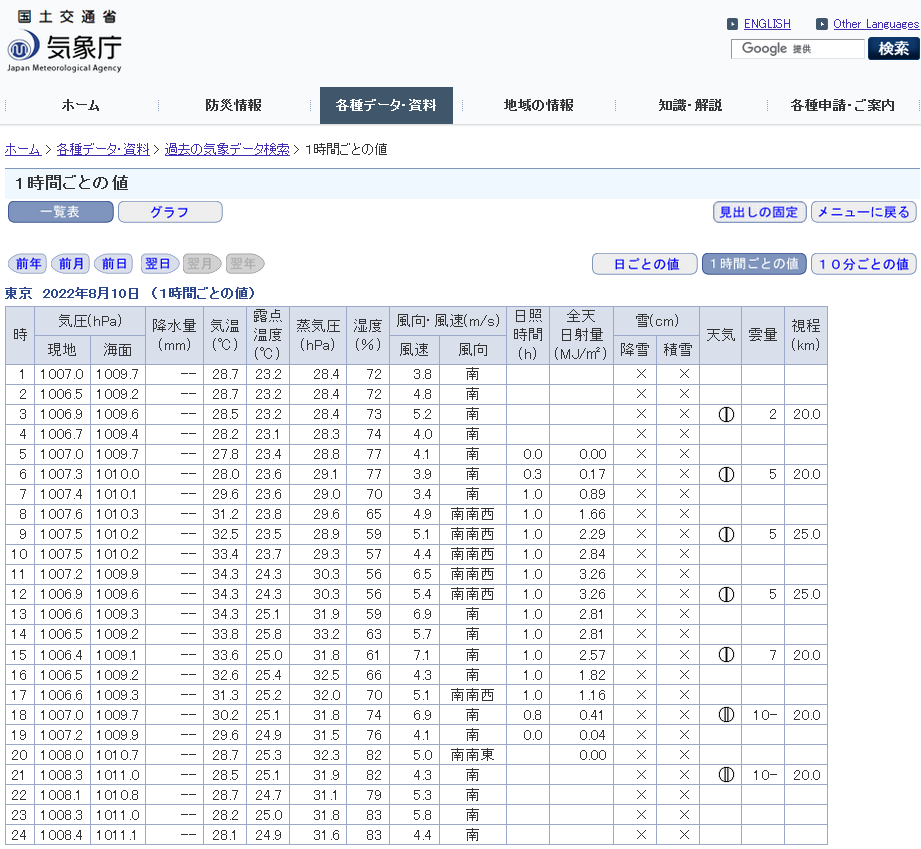
\includegraphics{../fig/JMA.png}
\caption{出典:気象庁|過去の気象データ検索}
\end{figure}

\hypertarget{urlux89e3ux6790}{%
\section{URL解析}\label{urlux89e3ux6790}}

取得したいデータがあるウェブページのURLを見てどのような規則で表示されているかを推察する.

\begin{verbatim}
https://www.data.jma.go.jp/obd/stats/etrn/view/hourly_s1.php?prec_no=44&block_no=47662&year=2022&month=8&day=10&view=  
\end{verbatim}

この例では,prec\_no,block\_noは正確には分からないが恐らく気象観測所に関する番号であろう,year,month,dayが年月日だろうと当たりが付く.このようにパラメータを含む形でURLが記載されている場合は,パラメータをプログラムで変えることで異なるウェブページに機械的にアクセスできる.

\hypertarget{ux8a2dux5b9a}{%
\section{設定}\label{ux8a2dux5b9a}}

\begin{Shaded}
\begin{Highlighting}[]
\CommentTok{\# 出力ファイル}
\NormalTok{DB  }\OtherTok{\textless{}{-}} \StringTok{\textquotesingle{}weather.db\textquotesingle{}}  \CommentTok{\# データベース名}
\NormalTok{F.O }\OtherTok{\textless{}{-}} \StringTok{\textquotesingle{}weather.csv\textquotesingle{}} \CommentTok{\# CSVファイル名}

\CommentTok{\# 気象観測所}
\NormalTok{site }\OtherTok{\textless{}{-}} \FunctionTok{data.frame}\NormalTok{(}
  \AttributeTok{id   =} \DecValTok{47662}\NormalTok{,   }\CommentTok{\# 番号}
  \AttributeTok{name =} \StringTok{\textquotesingle{}Tokyo\textquotesingle{}}\NormalTok{) }\CommentTok{\# 名称(データベースのテーブル名として使う)}

\CommentTok{\# システムロケール(海外クラウド環境利用時に必要な時間と言語の設定)}
\FunctionTok{Sys.setlocale}\NormalTok{(}\StringTok{"LC\_TIME"}\NormalTok{, }\StringTok{"ja\_JP.UTF{-}8"}\NormalTok{)}
\end{Highlighting}
\end{Shaded}

\begin{verbatim}
## [1] "ja_JP.UTF-8"
\end{verbatim}

\begin{Shaded}
\begin{Highlighting}[]
\CommentTok{\# 対象日時(テーブル取得のためのURLに適用する日時)}
\NormalTok{lt }\OtherTok{\textless{}{-}} \FunctionTok{as.POSIXlt}\NormalTok{(}\StringTok{\textquotesingle{}2022{-}08{-}10\textquotesingle{}}\NormalTok{) }\CommentTok{\# POSIX準拠ローカル時間}
\NormalTok{year  }\OtherTok{\textless{}{-}} \DecValTok{1900} \SpecialCharTok{+}\NormalTok{ lt}\SpecialCharTok{$}\NormalTok{year}
\NormalTok{month }\OtherTok{\textless{}{-}} \DecValTok{1} \SpecialCharTok{+}\NormalTok{ lt}\SpecialCharTok{$}\NormalTok{mon}
\NormalTok{day   }\OtherTok{\textless{}{-}}\NormalTok{ lt}\SpecialCharTok{$}\NormalTok{mday}
\end{Highlighting}
\end{Shaded}

\hypertarget{urlux4f5cux6210}{%
\section{URL作成}\label{urlux4f5cux6210}}

\begin{Shaded}
\begin{Highlighting}[]
\NormalTok{url }\OtherTok{\textless{}{-}} \FunctionTok{paste0}\NormalTok{(}\StringTok{\textquotesingle{}https://www.data.jma.go.jp/obd/stats/etrn/view/hourly\_s1.php?prec\_no=44\&block\_no=\textquotesingle{}}\NormalTok{, site}\SpecialCharTok{$}\NormalTok{id, }\StringTok{\textquotesingle{}\&year=\textquotesingle{}}\NormalTok{, year, }\StringTok{\textquotesingle{}\&month=\textquotesingle{}}\NormalTok{, month, }\StringTok{\textquotesingle{}\&day=\textquotesingle{}}\NormalTok{, day, }\StringTok{\textquotesingle{}\&view=\textquotesingle{}}\NormalTok{)}
\end{Highlighting}
\end{Shaded}

\hypertarget{ux30a6ux30a7ux30d6ux30daux30fcux30b8ux306eux30c7ux30fcux30bfux53d6ux5f97-web-scraping}{%
\section{ウェブページのデータ取得 (Web
scraping)}\label{ux30a6ux30a7ux30d6ux30daux30fcux30b8ux306eux30c7ux30fcux30bfux53d6ux5f97-web-scraping}}

\hypertarget{ux30c6ux30fcux30d6ux30ebux53d6ux5f97}{%
\subsection{テーブル取得}\label{ux30c6ux30fcux30d6ux30ebux53d6ux5f97}}

\begin{Shaded}
\begin{Highlighting}[]
\FunctionTok{library}\NormalTok{(rvest)}
\NormalTok{tbl }\OtherTok{\textless{}{-}} \FunctionTok{read\_html}\NormalTok{(url) }\SpecialCharTok{\%\textgreater{}\%} \FunctionTok{html\_table}\NormalTok{()}
\NormalTok{tbl}
\end{Highlighting}
\end{Shaded}

\begin{verbatim}
## [[1]]
## # A tibble: 1 x 2
##   X1    X2   
##   <lgl> <lgl>
## 1 NA    NA   
## 
## [[2]]
## # A tibble: 1 x 2
##   X1    X2   
##   <lgl> <lgl>
## 1 NA    NA   
## 
## [[3]]
## # A tibble: 1 x 7
##   X1    X2    X3    X4    X5    X6    X7   
##   <lgl> <lgl> <lgl> <lgl> <lgl> <lgl> <lgl>
## 1 NA    NA    NA    NA    NA    NA    NA   
## 
## [[4]]
## # A tibble: 1 x 3
##   X1    X2    X3   
##   <lgl> <lgl> <lgl>
## 1 NA    NA    NA   
## 
## [[5]]
## # A tibble: 25 x 17
##    時    気圧(~1 気圧(~2 降水~3  気温(~4 露点~5  蒸気~6  湿度(~7 風向~8 風向・~9
##    <chr> <chr>   <chr>   <chr>   <chr>   <chr>   <chr>   <chr>   <chr>  <chr>   
##  1 時    現地    海面    降水量~ 気温(℃) 露点温~ 蒸気圧~ 湿度(~  風速   風向    
##  2 1     1007.0  1009.7  --      28.7    23.2    28.4    72      3.8    南      
##  3 2     1006.5  1009.2  --      28.7    23.2    28.4    72      4.8    南      
##  4 3     1006.9  1009.6  --      28.5    23.2    28.4    73      5.2    南      
##  5 4     1006.7  1009.4  --      28.2    23.1    28.3    74      4.0    南      
##  6 5     1007.0  1009.7  --      27.8    23.4    28.8    77      4.1    南      
##  7 6     1007.3  1010.0  --      28.0    23.6    29.1    77      3.9    南      
##  8 7     1007.4  1010.1  --      29.6    23.6    29.0    70      3.4    南      
##  9 8     1007.6  1010.3  --      31.2    23.8    29.6    65      4.9    南南西  
## 10 9     1007.5  1010.2  --      32.5    23.5    28.9    59      5.1    南南西  
## # ... with 15 more rows, 7 more variables: `日照時間(h)` <chr>,
## #   `全天日射量(MJ/㎡)` <chr>, `雪(cm)` <chr>, `雪(cm)` <chr>, 天気 <chr>,
## #   雲量 <chr>, `視程(km)` <chr>, and abbreviated variable names
## #   1: `気圧(hPa)`, 2: `気圧(hPa)`, 3: `降水量(mm)`, 4: `気温(℃)`,
## #   5: `露点温度(℃)`, 6: `蒸気圧(hPa)`, 7: `湿度(%)`, 8: `風向・風速(m/s)`,
## #   9: `風向・風速(m/s)`
## # i Use `print(n = ...)` to see more rows, and `colnames()` to see all variable names
## 
## [[6]]
## # A tibble: 1 x 1
##   X1   
##   <chr>
## 1 -- 
## 
## [[7]]
## # A tibble: 1 x 4
##   X1             X2                  X3                 X4                  
##   <chr>          <chr>               <chr>              <chr>               
## 1 利用される方へ よくある質問(FAQ) 気象観測統計の解説 年・季節・各月の天候
\end{verbatim}

tblをプリントし,どのテーブルに必要なデータが格納されているか確認すると5番目のテーブル(リスト)にあることが分かる.
次で5番目のリストを取り出す.すべてテキストデータ(chr)になっている.

\begin{Shaded}
\begin{Highlighting}[]
\NormalTok{d0 }\OtherTok{\textless{}{-}} \FunctionTok{as.data.frame}\NormalTok{(tbl[[}\DecValTok{5}\NormalTok{]])}
\FunctionTok{str}\NormalTok{(d0)}
\end{Highlighting}
\end{Shaded}

\begin{verbatim}
## 'data.frame':    25 obs. of  17 variables:
##  $ 時               : chr  "時" "1" "2" "3" ...
##  $ 気圧(hPa)        : chr  "現地" "1007.0" "1006.5" "1006.9" ...
##  $ 気圧(hPa)        : chr  "海面" "1009.7" "1009.2" "1009.6" ...
##  $ 降水量(mm)       : chr  "降水量(mm)" "--" "--" "--" ...
##  $ 気温(℃)         : chr  "気温(℃)" "28.7" "28.7" "28.5" ...
##  $ 露点温度(℃)     : chr  "露点温度(℃)" "23.2" "23.2" "23.2" ...
##  $ 蒸気圧(hPa)      : chr  "蒸気圧(hPa)" "28.4" "28.4" "28.4" ...
##  $ 湿度(%)         : chr  "湿度(%)" "72" "72" "73" ...
##  $ 風向・風速(m/s)  : chr  "風速" "3.8" "4.8" "5.2" ...
##  $ 風向・風速(m/s)  : chr  "風向" "南" "南" "南" ...
##  $ 日照時間(h)      : chr  "日照時間(h)" "" "" "" ...
##  $ 全天日射量(MJ/㎡): chr  "全天日射量(MJ/㎡)" "" "" "" ...
##  $ 雪(cm)           : chr  "降雪" "×" "×" "×" ...
##  $ 雪(cm)           : chr  "積雪" "×" "×" "×" ...
##  $ 天気             : chr  "天気" "" "" "" ...
##  $ 雲量             : chr  "雲量" "" "" "2" ...
##  $ 視程(km)         : chr  "視程(km)" "" "" "20.0" ...
\end{verbatim}

\hypertarget{ux30c6ux30fcux30d6ux30ebux306eux6574ux5f62}{%
\subsection{テーブルの整形}\label{ux30c6ux30fcux30d6ux30ebux306eux6574ux5f62}}

日時などの情報追加,変数の型指定,データの整形を行い,書込用テーブルを作成する.
日時のフォーマット(\%Y-\%m-\%d
\%H:\%M:\%Sなど)はどのプログラミング言語でもほぼ共通なのでしっかりと記憶しておくこと.Rコンソールで「?strptime」とタイプすれば他の記号も調べることができる.

\begin{Shaded}
\begin{Highlighting}[]
\CommentTok{\# 日時整形}
\NormalTok{hour }\OtherTok{\textless{}{-}}\NormalTok{ d0[}\SpecialCharTok{{-}}\DecValTok{1}\NormalTok{, }\StringTok{\textquotesingle{}時\textquotesingle{}}\NormalTok{] }\CommentTok{\# 1列目は時刻1~24({-}1:一行目は不要なため削除)}
\CommentTok{\# コンピュータの世界(POSIX準拠)では24時は存在しないので0~23にする必要がある.}
\CommentTok{\# コンピュータ上では24時は翌日の日付になる.}
\NormalTok{datetime }\OtherTok{\textless{}{-}} \FunctionTok{as.POSIXlt}\NormalTok{(}\FunctionTok{paste}\NormalTok{(lt, hour),        }\CommentTok{\# 例)2022{-}08{-}10 24}
                       \AttributeTok{format =} \StringTok{\textquotesingle{}\%Y{-}\%m{-}\%d \%H\textquotesingle{}}\NormalTok{) }\CommentTok{\# 例の様な数字を「年{-}月{-}日 時」として読込む}
                                               \CommentTok{\# 自動で時刻が0~23に変換される.}

\CommentTok{\# 書込用テーブル作成}
\NormalTok{d1 }\OtherTok{\textless{}{-}} \FunctionTok{data.frame}\NormalTok{(}\AttributeTok{site.id   =} \FunctionTok{as.integer}\NormalTok{(site}\SpecialCharTok{$}\NormalTok{id), }\CommentTok{\# 整数型}
                 \AttributeTok{site.name =}\NormalTok{ site}\SpecialCharTok{$}\NormalTok{name,}
                 \AttributeTok{datetime  =} \FunctionTok{format}\NormalTok{(datetime, }\StringTok{\textquotesingle{}\%Y{-}\%m{-}\%d \%H:00\textquotesingle{}}\NormalTok{),}
                 \AttributeTok{temp      =} \FunctionTok{as.double}\NormalTok{(d0[}\SpecialCharTok{{-}}\DecValTok{1}\NormalTok{, }\DecValTok{5}\NormalTok{]), }\CommentTok{\# 倍精度浮動小数点型}
                 \AttributeTok{wind      =}\NormalTok{ d0[}\SpecialCharTok{{-}}\DecValTok{1}\NormalTok{, }\DecValTok{10}\NormalTok{])}
\FunctionTok{str}\NormalTok{(d1)}
\end{Highlighting}
\end{Shaded}

\begin{verbatim}
## 'data.frame':    24 obs. of  5 variables:
##  $ site.id  : int  47662 47662 47662 47662 47662 47662 47662 47662 47662 47662 ...
##  $ site.name: chr  "Tokyo" "Tokyo" "Tokyo" "Tokyo" ...
##  $ datetime : chr  "2022-08-10 01:00" "2022-08-10 02:00" "2022-08-10 03:00" "2022-08-10 04:00" ...
##  $ temp     : num  28.7 28.7 28.5 28.2 27.8 28 29.6 31.2 32.5 33.4 ...
##  $ wind     : chr  "南" "南" "南" "南" ...
\end{verbatim}

\hypertarget{ux30c7ux30fcux30bfux4fddux5b58}{%
\section{データ保存}\label{ux30c7ux30fcux30bfux4fddux5b58}}

\hypertarget{ux30c7ux30fcux30bfux30d9ux30fcux30b9sqliteux3078ux306eux4fddux5b58}{%
\subsection{データベース(SQLite)への保存}\label{ux30c7ux30fcux30bfux30d9ux30fcux30b9sqliteux3078ux306eux4fddux5b58}}

\begin{Shaded}
\begin{Highlighting}[]
\FunctionTok{library}\NormalTok{(RSQLite)}

\CommentTok{\# データベース接続}
\NormalTok{conn }\OtherTok{\textless{}{-}} \FunctionTok{dbConnect}\NormalTok{(RSQLite}\SpecialCharTok{::}\FunctionTok{SQLite}\NormalTok{(), DB)}

\CommentTok{\# 既存テーブル削除(必要に応じて実施)}
\FunctionTok{dbSendQuery}\NormalTok{(conn, }\FunctionTok{paste}\NormalTok{(}\StringTok{\textquotesingle{}DROP TABLE IF EXISTS\textquotesingle{}}\NormalTok{, site}\SpecialCharTok{$}\NormalTok{name))}
\end{Highlighting}
\end{Shaded}

\begin{verbatim}
## <SQLiteResult>
##   SQL  DROP TABLE IF EXISTS Tokyo
##   ROWS Fetched: 0 [complete]
##        Changed: 0
\end{verbatim}

\begin{Shaded}
\begin{Highlighting}[]
\CommentTok{\# テーブル追記書込}
\FunctionTok{dbWriteTable}\NormalTok{(conn, site}\SpecialCharTok{$}\NormalTok{name, d1, }\AttributeTok{append =}\NormalTok{ T)}
\end{Highlighting}
\end{Shaded}

レコードを重複して保存したくない場合は,レコードがユニークになるように
PRIMARY KEYを設定するとよい.DB Browser for
SQLiteなどのGUIツールを使うと簡単に設定できる.設定すると重複するレコードが来たときにプログラムはエラー停止する.繰返計算などで停止させたくないときはtry()関数を付けるとプログラム実行を継続できる.

\begin{figure}
\centering
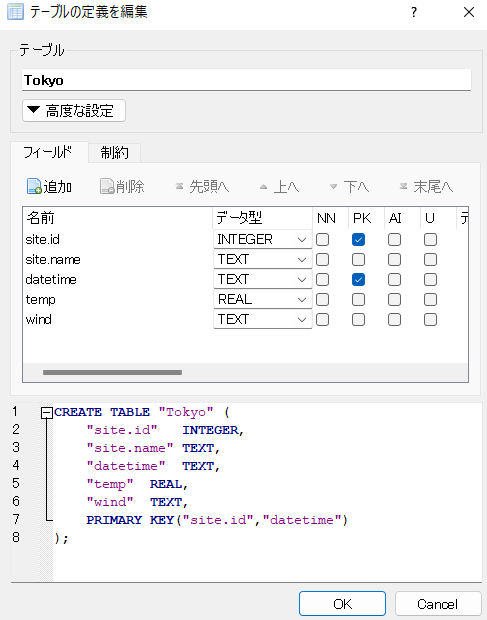
\includegraphics{../fig/db_browser_table_def.png}
\caption{PRIMARY KEYの設定例(DB Browser for SQLite)}
\end{figure}

複数のカラムを組み合わせたPRIMARY
KEY(PK)とすることでレコードがユニークになる.また,データハンドリングも高速になる利点もある.

\begin{Shaded}
\begin{Highlighting}[]
\CommentTok{\# データ選択(ちゃんと保存されたか確認すること)}
\NormalTok{res }\OtherTok{\textless{}{-}} \FunctionTok{dbSendQuery}\NormalTok{(conn, }\StringTok{\textquotesingle{}SELECT * FROM Tokyo WHERE wind = "南"\textquotesingle{}}\NormalTok{)}

\CommentTok{\# 選択結果取得}
\FunctionTok{dbFetch}\NormalTok{(res)}
\end{Highlighting}
\end{Shaded}

\begin{verbatim}
##    site.id site.name         datetime temp wind
## 1    47662     Tokyo 2022-08-10 01:00 28.7   南
## 2    47662     Tokyo 2022-08-10 02:00 28.7   南
## 3    47662     Tokyo 2022-08-10 03:00 28.5   南
## 4    47662     Tokyo 2022-08-10 04:00 28.2   南
## 5    47662     Tokyo 2022-08-10 05:00 27.8   南
## 6    47662     Tokyo 2022-08-10 06:00 28.0   南
## 7    47662     Tokyo 2022-08-10 07:00 29.6   南
## 8    47662     Tokyo 2022-08-10 13:00 34.3   南
## 9    47662     Tokyo 2022-08-10 14:00 33.8   南
## 10   47662     Tokyo 2022-08-10 15:00 33.6   南
## 11   47662     Tokyo 2022-08-10 16:00 32.6   南
## 12   47662     Tokyo 2022-08-10 18:00 30.2   南
## 13   47662     Tokyo 2022-08-10 19:00 29.6   南
## 14   47662     Tokyo 2022-08-10 21:00 28.5   南
## 15   47662     Tokyo 2022-08-10 22:00 28.7   南
## 16   47662     Tokyo 2022-08-10 23:00 28.2   南
## 17   47662     Tokyo 2022-08-11 00:00 28.1   南
\end{verbatim}

\begin{Shaded}
\begin{Highlighting}[]
\CommentTok{\# 選択結果解放}
\FunctionTok{dbClearResult}\NormalTok{(res)}

\CommentTok{\# データベース接続解除 }
\FunctionTok{dbDisconnect}\NormalTok{(conn)}
\end{Highlighting}
\end{Shaded}

\hypertarget{csvux30d5ux30a1ux30a4ux30ebux3078ux306eux4fddux5b58}{%
\subsection{CSVファイルへの保存}\label{csvux30d5ux30a1ux30a4ux30ebux3078ux306eux4fddux5b58}}

\begin{Shaded}
\begin{Highlighting}[]
\CommentTok{\# 既存ファイル削除(必要に応じて実施)}
\FunctionTok{file.remove}\NormalTok{(F.O)}
\end{Highlighting}
\end{Shaded}

\begin{verbatim}
## [1] TRUE
\end{verbatim}

\begin{Shaded}
\begin{Highlighting}[]
\CommentTok{\# テーブル追記書込}
\FunctionTok{library}\NormalTok{(data.table)}
\FunctionTok{fwrite}\NormalTok{(d1, }\AttributeTok{file =}\NormalTok{ F.O, }\AttributeTok{sep =} \StringTok{\textquotesingle{},\textquotesingle{}}\NormalTok{, }\AttributeTok{append =}\NormalTok{ T)}
\end{Highlighting}
\end{Shaded}

\begin{Shaded}
\begin{Highlighting}[]
\CommentTok{\# 読込確認}
\NormalTok{(d2 }\OtherTok{\textless{}{-}} \FunctionTok{fread}\NormalTok{(}\AttributeTok{file =}\NormalTok{ F.O))}
\end{Highlighting}
\end{Shaded}

\begin{verbatim}
##     site.id site.name         datetime temp   wind
##  1:   47662     Tokyo 2022-08-10 01:00 28.7     南
##  2:   47662     Tokyo 2022-08-10 02:00 28.7     南
##  3:   47662     Tokyo 2022-08-10 03:00 28.5     南
##  4:   47662     Tokyo 2022-08-10 04:00 28.2     南
##  5:   47662     Tokyo 2022-08-10 05:00 27.8     南
##  6:   47662     Tokyo 2022-08-10 06:00 28.0     南
##  7:   47662     Tokyo 2022-08-10 07:00 29.6     南
##  8:   47662     Tokyo 2022-08-10 08:00 31.2 南南西
##  9:   47662     Tokyo 2022-08-10 09:00 32.5 南南西
## 10:   47662     Tokyo 2022-08-10 10:00 33.4 南南西
## 11:   47662     Tokyo 2022-08-10 11:00 34.3 南南西
## 12:   47662     Tokyo 2022-08-10 12:00 34.3 南南西
## 13:   47662     Tokyo 2022-08-10 13:00 34.3     南
## 14:   47662     Tokyo 2022-08-10 14:00 33.8     南
## 15:   47662     Tokyo 2022-08-10 15:00 33.6     南
## 16:   47662     Tokyo 2022-08-10 16:00 32.6     南
## 17:   47662     Tokyo 2022-08-10 17:00 31.3 南南西
## 18:   47662     Tokyo 2022-08-10 18:00 30.2     南
## 19:   47662     Tokyo 2022-08-10 19:00 29.6     南
## 20:   47662     Tokyo 2022-08-10 20:00 28.7 南南東
## 21:   47662     Tokyo 2022-08-10 21:00 28.5     南
## 22:   47662     Tokyo 2022-08-10 22:00 28.7     南
## 23:   47662     Tokyo 2022-08-10 23:00 28.2     南
## 24:   47662     Tokyo 2022-08-11 00:00 28.1     南
##     site.id site.name         datetime temp   wind
\end{verbatim}

\end{document}
